% !TeX root = ../sustechthesis-example.tex

\chapter[激光功率稳定]{激光功率稳定}
\section[激光功率稳定]{激光功率稳定}
在离子阱量子计算中,激光功率稳定非常重要,因为激光功率的波动会影响离子阱中囚禁离子的运动和量子态\cite[]{Blums_Scarabel_Shimizu_Ghadimi_Connell_Händel_Norton_Bridge_Kielpinski_Lobino_et_al_2020}。具体来说,激光功率稳定有以下几个作用:
\begin{enumerate}
    \item 提高量子比特的质量:激光功率稳定可以减少离子阱中囚禁离子的运动和量子态的噪声,从而提高量子比特的质量和精度;
    \item 延长量子比特的寿命:激光功率稳定可以减少离子阱中囚禁离子的能量损失,从而延长量子比特的寿命;
    \item 提高量子计算的成功率:激光功率稳定可以减少离子阱中囚禁离子的运动和量子态的噪声,从而提高量子计算的成功率;
    \item 实现精确的量子操作:激光功率稳定可以实现精确的量子操作,例如囚禁离子的冷却、囚禁离子的量子门操作等;
    \item 
\end{enumerate}

因此,在离子阱量子计算中,保持激光功率稳定是非常重要的,可以提高量子比特的质量、延长量子比特的寿命、提高量子计算的成功率和实现精确的量子操作。



\section[激光功率外部稳定原理]{激光功率外部稳定原理}
激光功率稳定与多种因素有关,通常来说有温度控制、电流控制、光学反馈控制、机械稳定性等,这些因素基本都针对激光器本身进行稳定。除了对激光器本身进行稳定外,还可以激光输出的后续光路中设计相关的控制系统对激光进行稳定。这种方式独立于激光器吱声的出光稳定,可以在激光出光稳定的基础上进一步提高激光功率的稳定性。下面介绍这种激光功率外部稳定原理和实现。

\begin{figure}
    \centering
    \caption[激光功率外部稳定]{激光功率外部稳定\label{fig:laser_stabilization0}}
    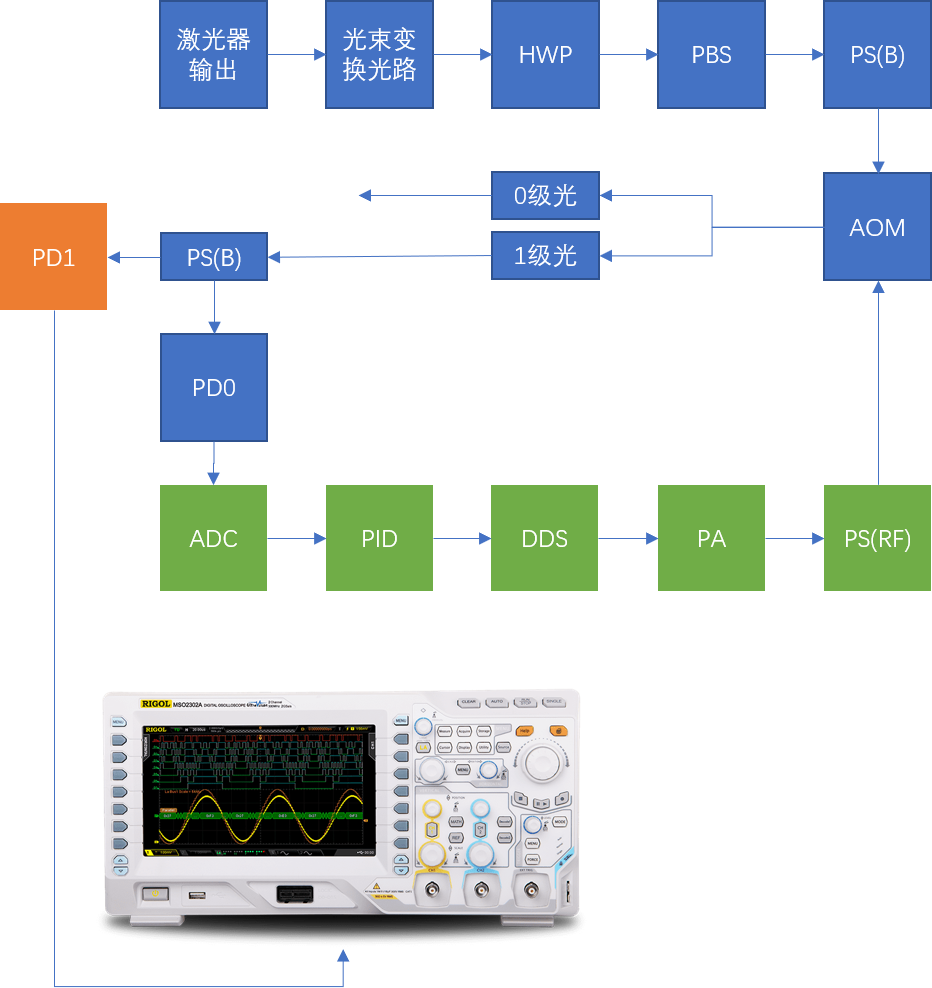
\includegraphics[width=1.0\linewidth]{laser_stabilization0}
\end{figure}

整个激光功率外部稳定系统主要包括如图\ref{fig:laser_stabilization0}几部分:激光器、透镜组、半波片HWP、光偏振分束镜PBS、光功率分配镜PS(B)、声光调制器AOM、光分束镜PS(B)、光子探测器PD、ADC芯片、数字PID、直接数字信号合成器DDS、射频功放PA、射频功率分配器PS(RF)。

整个过程如下,首先激光器产生激光经过透镜和反光镜组将激光变换到要求的光斑大小和入射位置;接着使用半波片(HWP)将光转化为垂直和水平偏振成分;接着使用偏振分数器将偏振光提纯为匹配AOM偏振需求的光;随后使用光功率分配器分出一部分激光用于构成反馈回路,另一部分光经过控制回路控制的AOM调制后成为可用的功率稳定激光;激光经过AOM后会产生若干级衍射光,起哄主要能量集中在0级和1级衍射光上,我们可以选择其中一路来进行探测和稳定(这里选择1级光);将一级光经过光功率分束镜一部分作为测试监测,另一部分用于反馈控制回路中。控制器采用基于RTMQ板卡数字系统实现,主要器件为ADC、数字PID、DDS,除此之外还需要功率放大器(PA)和射频功率分配器(可选,如果只有一路则不用,实际使用中可以分出多路来调控多了AOM)。通过调节射频功率的大小可以控制AOM1级光和0级光的功率分布,在合理范围内,功率越大1激光分得的功率越高。数字PID根据1级衍射光的功率变化控制DDS输出不同功率的射频信号,从而实现对1级衍射激光的稳定。

对于整个控制回路,一般来说只需要分出两路如AOM0和AOM1,一路AOM0用来做功率稳定的反馈回路,另一路AOM1用来做工作光,然后可以拓展地在另一路后面添加光功率分配镜来获得更多路的稳定光,如附录图\ref{fig:laser_stabilization}所示。


\section[激光功率锁定系统搭建]{激光功率锁定系统搭建}
激光功率锁定系统测试如附录图\ref{fig:laser_stabilization_real}所示。


\section[激光功率锁定系统结果]{激光功率锁定系统结果}
% D:\Database\Files\2021-2024-研究生事件文件\2022-2023\研究\2023年4月13日-光功率稳定\2023年4月27日_光功率计测试数据

数据的测量采用如图所示的RIGOL示波器进行,在50kHz的采样率下采集约3.5s的数据。激光功率外部稳定本底、稳定前、稳定后原始数据如图\ref{fig:laser_stabilization_data}所示,从图中看可以看出PD在无激光输入的暗态下本底噪声较小。除此之外,可以看到经过稳定后的激光功率小于稳定前的激光功率,这其中的主要原因是稳定过程中AOM动态分离了部分激光功率。为了能够有效地对比稳定前后的效果,我们用各组数据的均值对功率测试的结果进行归一化处理$P_{norm}=P_{orignal}/mean(P_{orignal})$,结果如图\ref{fig:laser_stabilization_data0}所示。由于本底噪声过于接近0,因此本底噪声的归一化结果呈现发散状态,在这里不具有参考价值。从图\ref{fig:laser_stabilization_data0}中可以明显看出经过数字PID稳定系统后的功率更加稳定了。

\begin{figure}
    \centering
    \caption[激光功率外部稳定原始数据]{激光功率外部稳定本底、稳定前、稳定后原始数据\label{fig:laser_stabilization_data}}
    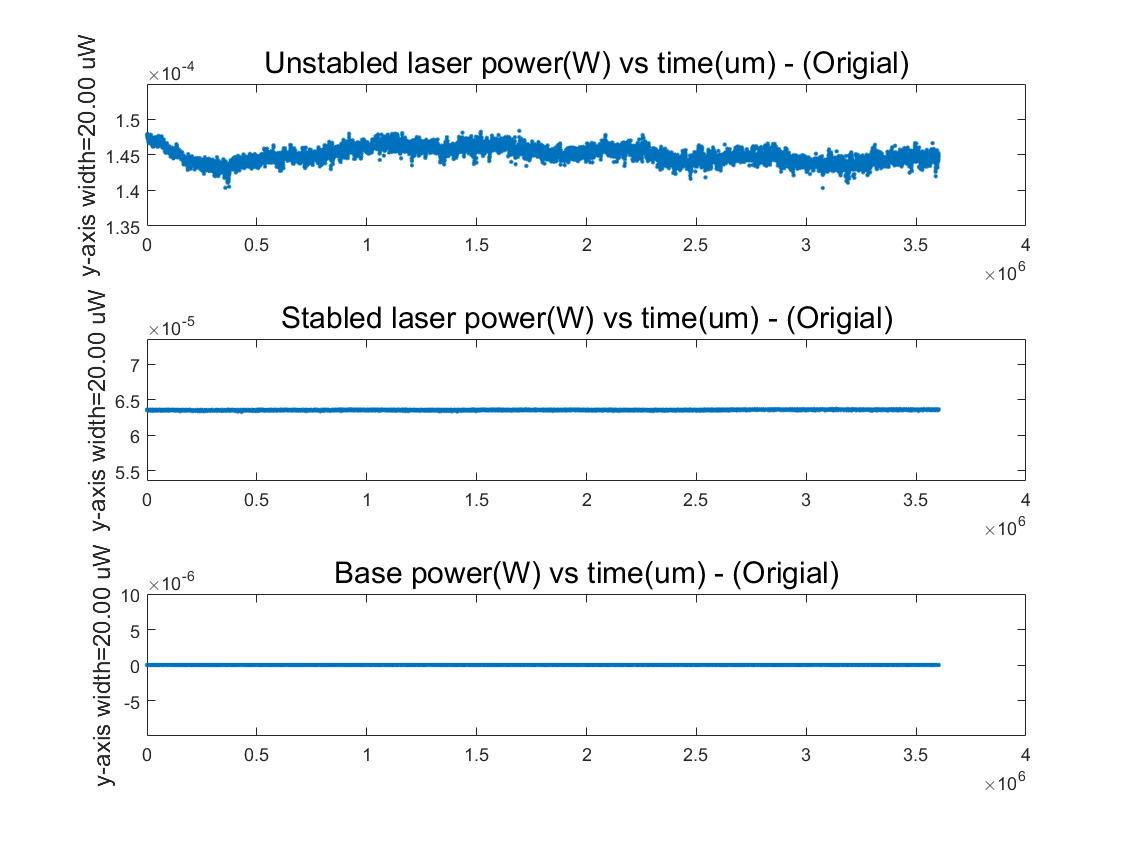
\includegraphics[width=1.0\linewidth]{laser_stabilization_data}
\end{figure}

\begin{figure}
    \centering
    \caption[激光功率外部稳定归一化后数据]{激光功率外部稳定归一化后本底、稳定前、稳定后数据\label{fig:laser_stabilization_data0}}
    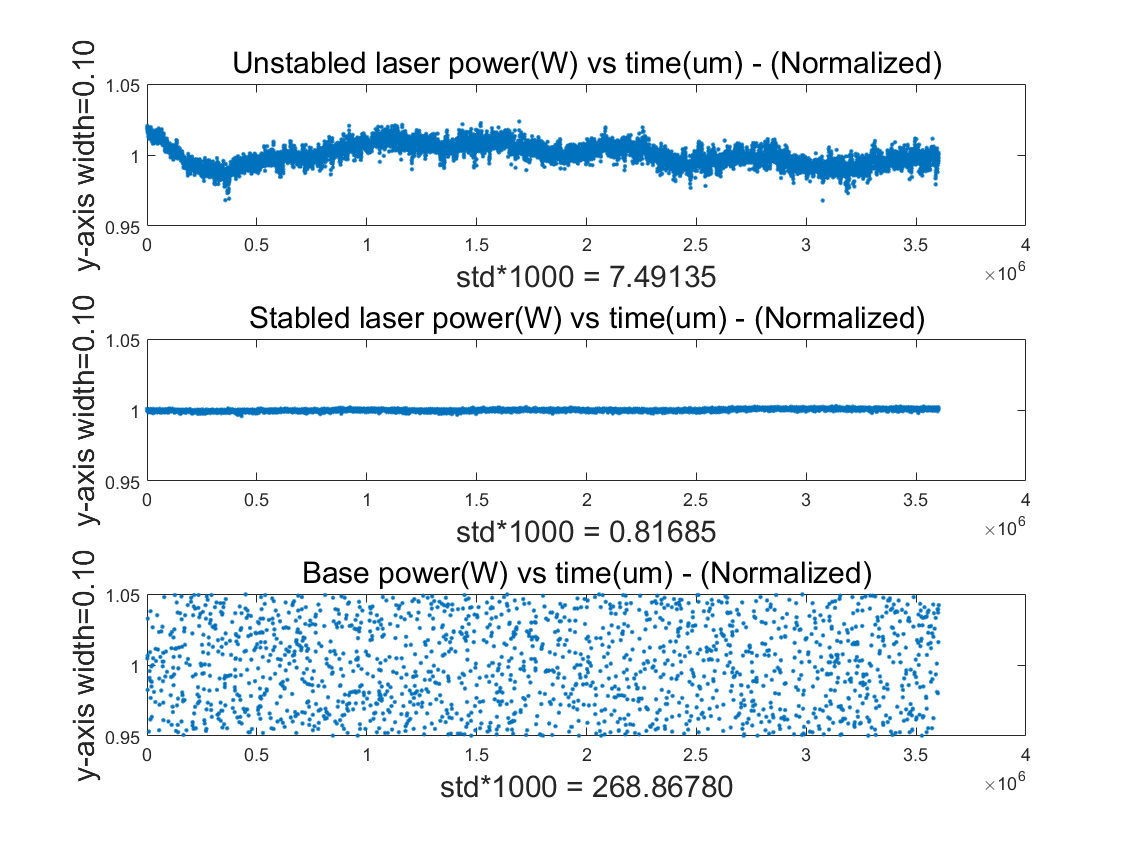
\includegraphics[width=1.0\linewidth]{laser_stabilization_data0}
\end{figure}

一般来说可以通过计算两组数据归一化后的方差之比可以粗略地获得稳定效果,方差越小稳定性越高。经计算稳定前后激光功率数据的方差比为$\frac{\sigma_{unstable}}{\sigma_{stabled}}\approx 9.17$。整体上经过激光功率稳定系统后,稳定前好了约9倍。为了能够更加直观地评估稳定的效果,我们将归一化后的所有数据点绘制出统计柱状图(由于本底的归一化不具有参考价值因此这里省略),结果如图\ref{fig:laser_stabilization_data1}所示。
\begin{figure}
    \centering
    \caption[激光功率外部稳定柱状图对比数据]{激光功率外部稳定归一化后本底、稳定前、稳定后数据柱状图。\label{fig:laser_stabilization_data1}}
    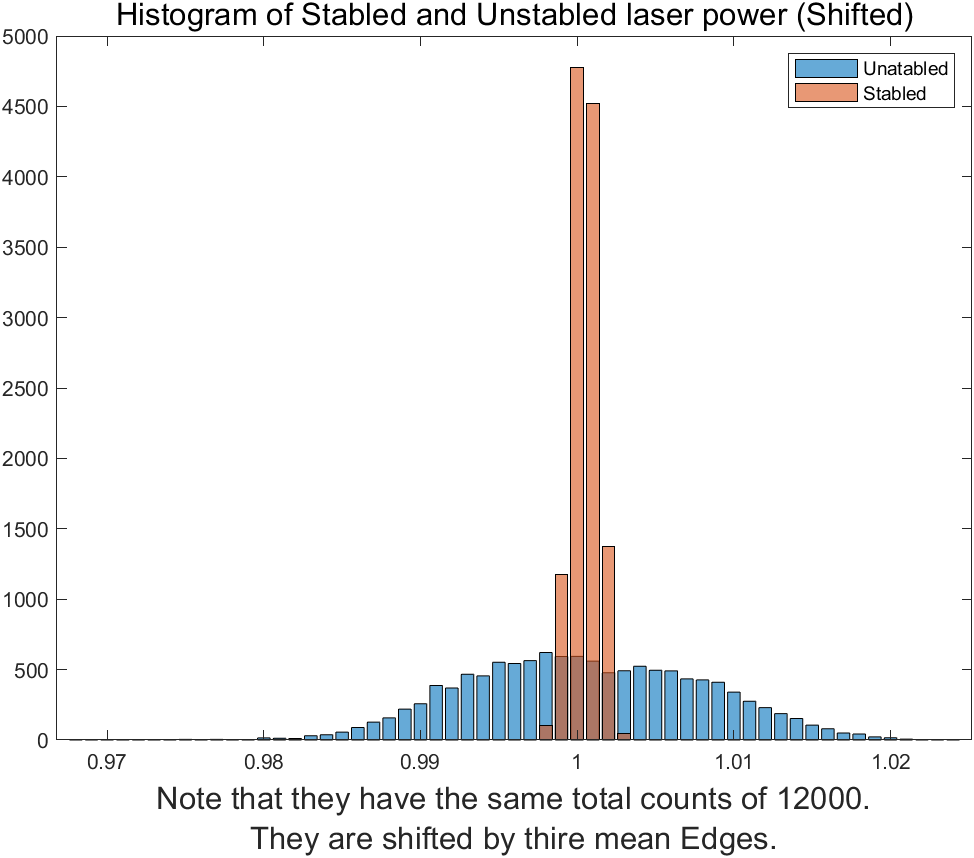
\includegraphics[width=0.8\linewidth]{laser_stabilization_data1}
\end{figure}

为了能更好了解稳定效果的长时间表现情况,我们重新以3Hz的采样率采集了一组长期数据,并绘制出了归一化后稳定前后数据的阿兰方差,如图\ref{fig:laser_stabilization_data2}所示。从结果对比来看,稳定后的激光功率数据的阿兰方差在各个滑动窗口都低于未稳定时的。表明这里的数字稳定系统在较长时间的各个滑动窗口稳定性都好于未稳定时的。
\begin{figure}
    \centering
    \caption[激光功率外部稳定阿兰方差对比数据]{激光功率外部稳定归一化后本底、稳定前、稳定后数据阿兰方差。\label{fig:laser_stabilization_data2}}
    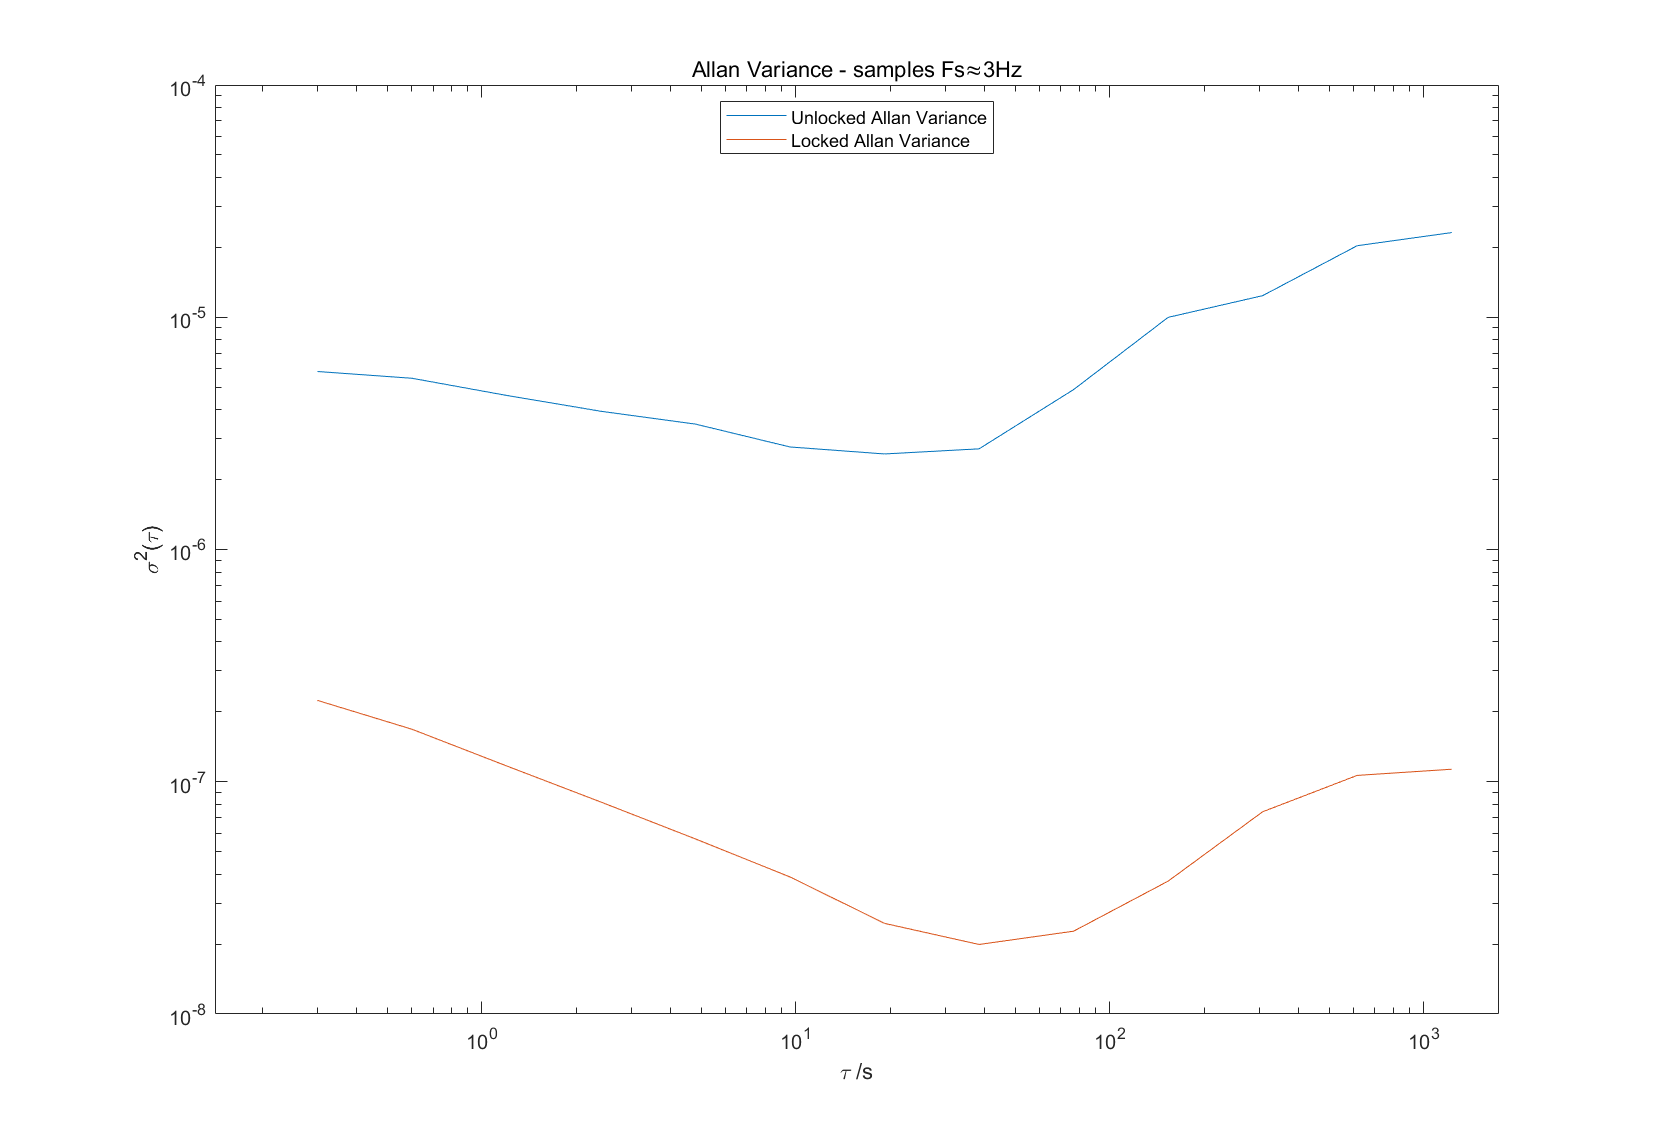
\includegraphics[width=0.8\linewidth]{laser_stabilization_data2}
\end{figure}


